\section{Ablation study}
\label{sec:ablation}

Additional experiments were performed on the ETTm1 datasets to analyze the different components of the Yformer model. Similar ablation experiment results for ETTh2 dataset are reported in the Appendix section for reference.

\subsection{Y-former architecture}

In this section, we attempt to understand (1) the improvement brought about by the Y-shaped model architecture, and (2) the impact of the reconstruction loss on the superiority of the Yformer model. Firstly, Figure \ref{fig:model_size_comparison} compares the model complexity for the proposed Yformer model with the Informer baseline model and demonstrates the advantage offered by the Yformer model for longer horizons. Secondly, Figures \ref{fig:ablation_archi_uni}, \ref{fig:ablation_archi_multi}, show that the Yformer architecture performs better or is comparable to the Informer throughout the entire horizon range. Moreover, for the larger horizons, the Yformer architecture without the reconstruction loss i.e. $\alpha=0$, has a clear advantage over the Informer baseline. We attribute this improvement in performance to the additional direct U-Net inspired connections within the Yformer architecture. Using feature maps at multiple resolutions offers a clear advantage by eliminating vanishing gradients and encouraging feature reuse. Figures \ref{fig:ablation_archi_uni}, \ref{fig:ablation_archi_multi} also clearly delineates the advantage offered by adding reconstruction loss as an auxiliary task for the model, by comparing Yformer with Yformer ($\alpha=0$) results. Such a multi-task approach offers regularization to the model by learning parameters that do not overfit on the future target distribution and propels the gradients towards a general distribution that can predict the history along with the future time steps.


\begin{figure}[t]
    \centering
    \begin{tabular}{c}
    
    \subfloat[ETTm1 Univariate\label{fig:ablation_archi_uni}]{%
      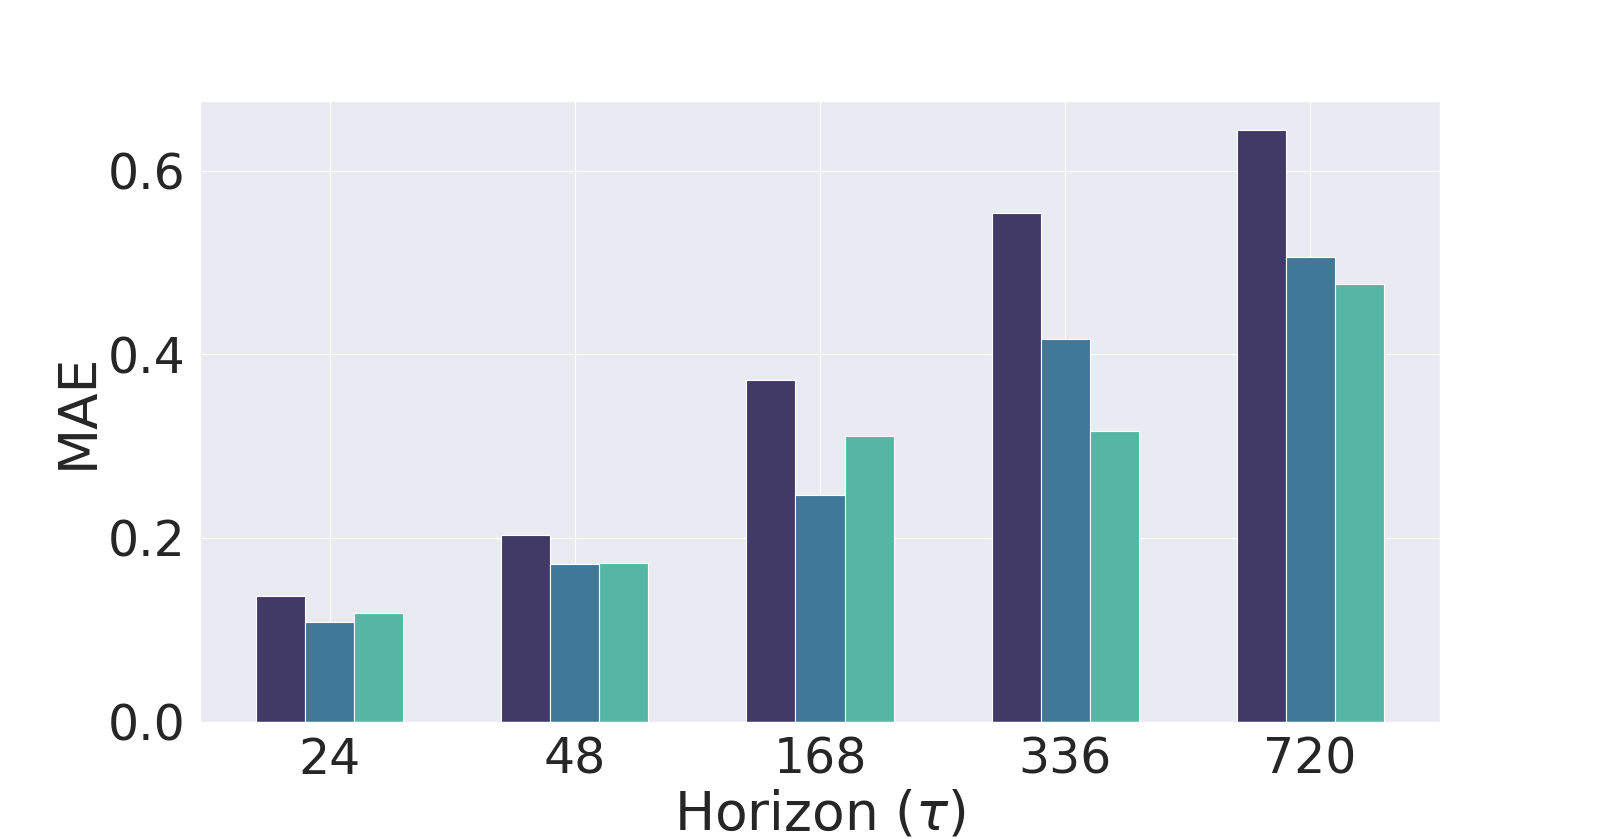
\includegraphics[width=0.40\textwidth]{figs/archi_ablation_uni_ETTm1.png}
    }

    \subfloat[ETTm1 Multivariate\label{fig:ablation_archi_multi}]{%
      \includegraphics[width=0.40\textwidth]{figs/archi_ablation_multi_ETTm1.png}
    }
    
    
    \\
    \subfloat[ETTm1 Univariate\label{fig:skipless_ablation_uni}]{%
      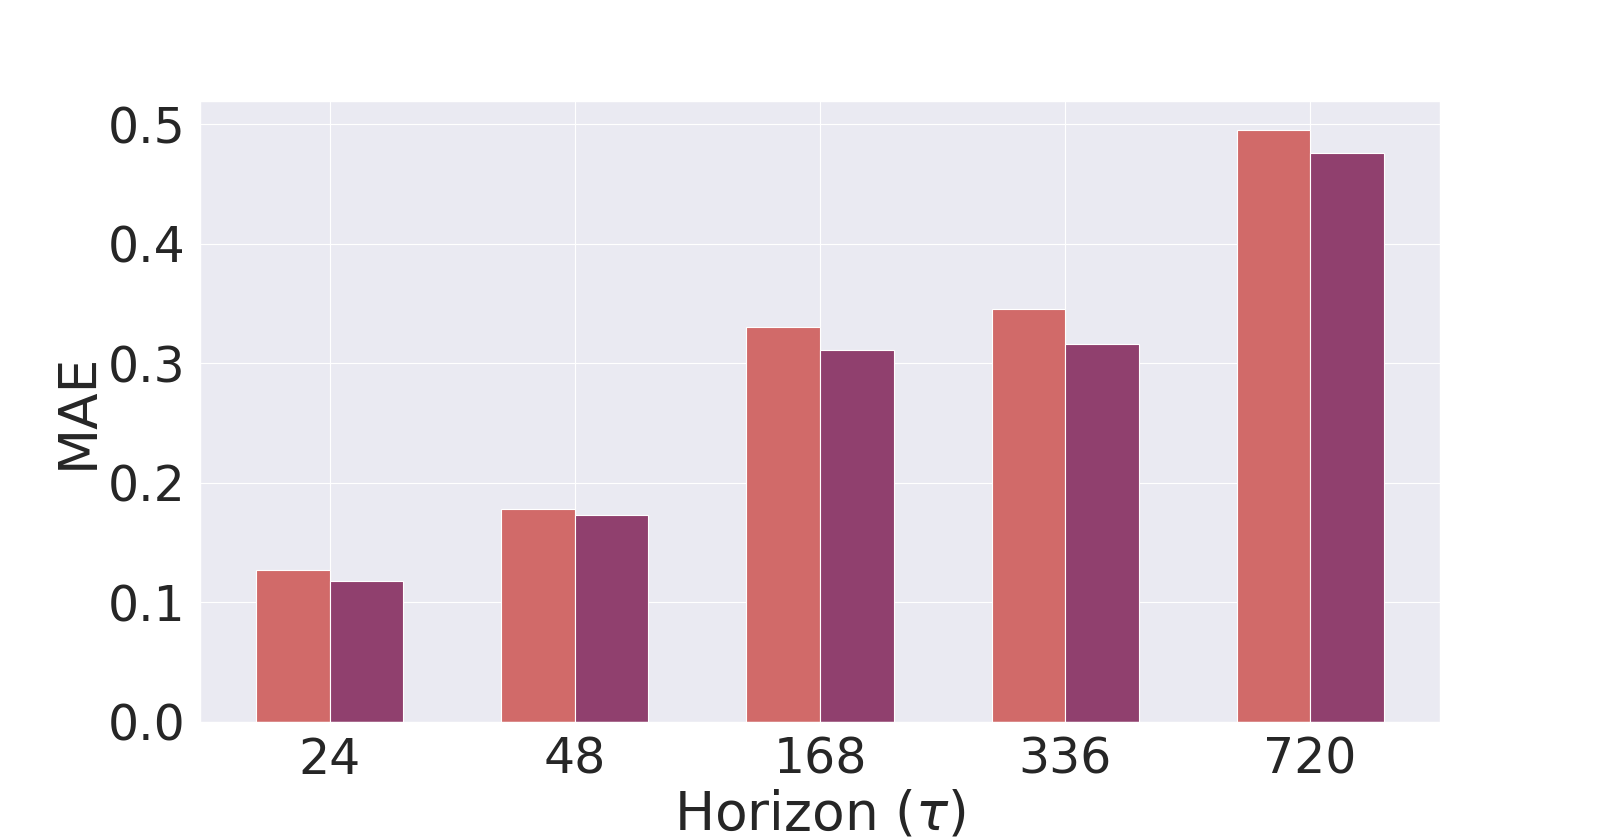
\includegraphics[width=0.40\textwidth]{figs/skipless_ablation_uni_updated.png}
    }
    \subfloat[ETTm1 Multivariate\label{fig:skipless_ablation_multi}]{%
      \includegraphics[width=0.40\textwidth]{figs/skipless_ablation_multi_updated.png}
    }
    \end{tabular}
\caption{(top) Figures \ref{fig:ablation_archi_uni}, \ref{fig:ablation_archi_multi} illustrates the reduction in MAE loss (y-axis) by  the Yformer architecture in comparison with the Informer baseline for the univariate and multivariate settings respectively. The Yformer ($\alpha=0$) represent the Yformer architecture without the reconstruction loss. (bottom) Figures \ref{fig:skipless_ablation_uni}, \ref{fig:skipless_ablation_multi} demonstrate the reduction in MAE loss (y-axis) brought by the addition of U-Net based skip connections (Yformer) to the Yformer architecture without the skip connections (Yformer$^*$). }
\label{fig:ablation_archi}
\end{figure}

\subsection{Effectiveness of the U-Net based skip connections}

To analyze the impact of U-Net based skip-connections, we conduct an ablation study on the Y-former architecture by removing the U-Net skip connections from the encoder to the decoder. We denote this model as Yformer$^*$. Figures \ref{fig:skipless_ablation_uni}, \ref{fig:skipless_ablation_multi} provides a summary of the results obtained after hyperparameter tuning the Yformer$^*$ and comparing it with the proposed Yformer model. The skip connections from the encoder to the decoder improve the performance throughout the entire horizon range for the multivariate setting and offers partial improvement for the univariate setting. Within the multivariate setting, the skip connections have a considerable impact on larger horizons and a smaller impact on the shorter horizons. This observation can be reasoned by considering the fact that long-range forecasting can utilize the additional multi-resolution encoder feature maps encoded by the U-Net based skip connections. Similar reason can be applied to the fact that U-Net based skip connections improve the performance of the multivariate setting more than that of the univariate settings.

\subsection{Reconstruction Factor}
\begin{figure}[t]
    \centering
    \begin{tabular}{c}
    \subfloat[best $\alpha$'s for Univariate\label{fig:alpha_ablation_uni}]{%
      \includegraphics[width=0.33\textwidth]{figs/factor_ablation_uni.png}
    }
    \subfloat[best $\alpha$'s for Multivariate\label{fig:alpha_ablation_multi}]{%
      \includegraphics[width=0.33\textwidth]{figs/factor_ablation_multi.png}
    }
    \subfloat[Model complexity\label{fig:model_size_comparison}]{%
      \includegraphics[width=0.34\textwidth]{figs/model_size_comparison.png}
    }
    \end{tabular}
\caption{Figures \ref{fig:alpha_ablation_uni} and \ref{fig:alpha_ablation_multi} illustrates the distribution of selected Reconstruction factor (y-axis) across the multiple horizons (x-axis). Figure \ref{fig:model_size_comparison}, compares the model size complexity (y-axis) for the multivariate setting across the multiple horizons (x-axis) for the Informer and the Yformer model.}
\label{fig:alpha_ablation}
\end{figure}


How impactful is the reconstruction factor $\alpha$ from the proposed loss in Eq. \ref{eqn:reconstruction}? We aggregated the optimal value chosen by hyperparameter tuning $\alpha$ across different datasets and summarized the distribution in Figures \ref{fig:alpha_ablation_uni} and \ref{fig:alpha_ablation_multi}. 
Interestingly, $\alpha$ value of $0.7$ is the predominant optimal setting across most horizons. Consequently, this shows that a high weight for the reconstruction loss helps the Yformer to achieve a lower loss for the future targets. Moreover, we can observe a trend that $\alpha$ is on average larger for short forecasting horizons signifying the importance of auxiliary loss for the shorter horizons. One possible reason could be that the reconstruction loss generalizes the output distribution better and avoids overfitting on short-horizon lengths. For the longer horizon forecasts, optimal $\alpha$ values are distributed on the lower and upper range of $\alpha$'s evenly, indicating that for long horizons, the reconstruction loss from long history helps for some datasets and does not for other datasets. This could be a characteristic of the dataset having a domain shift within the forecast horizon.

